\section{STL-Datenstrukturen}

\subsection{container adaptors}

\begin{frame}{Überblick - container adaptors}
 	\begin{block}{Adapter (Entwurfsmuster)}
	 	\pause
	 	Ausgangssituation: Eine Klasse bietet den erforderlichen Funktionsumfang, aber nicht (genau) die gewünschte Schnittstelle.
	 	
	 	\pause
	 	
	 	Ein Adapter:
	 	\begin{itemize}
	 		\item Übersetzt eine inkompatible Schnittstelle
	 		\item Wandelt ggf. die verwendeten Datenformate um
	 		\item Ist nach außen hin nicht als ein solcher erkennbar
	 	\end{itemize}
 	\end{block}
 	
 	\pause
 	
	\begin{itemize}
		\item \texttt{stack}
		\item \texttt{queue}
		\item \texttt{priority\_queue}
	\end{itemize}
	
	\pause
	
	\texttt{stack} und \texttt{queue} sind schon fast mehr Interface als eine vollwertige Klasse. Reicht deren Funktionsumfang aus, darf daher gerne deren Schnittstelle genutzt werden, was mehr Wahlfreiheit bei der Auswahl der zugrundeliegenden Datenstruktur erlaubt.
\end{frame}

\begin{frame}{\texttt{stack}}
	\begin{columns}
		\column{.3\linewidth}
			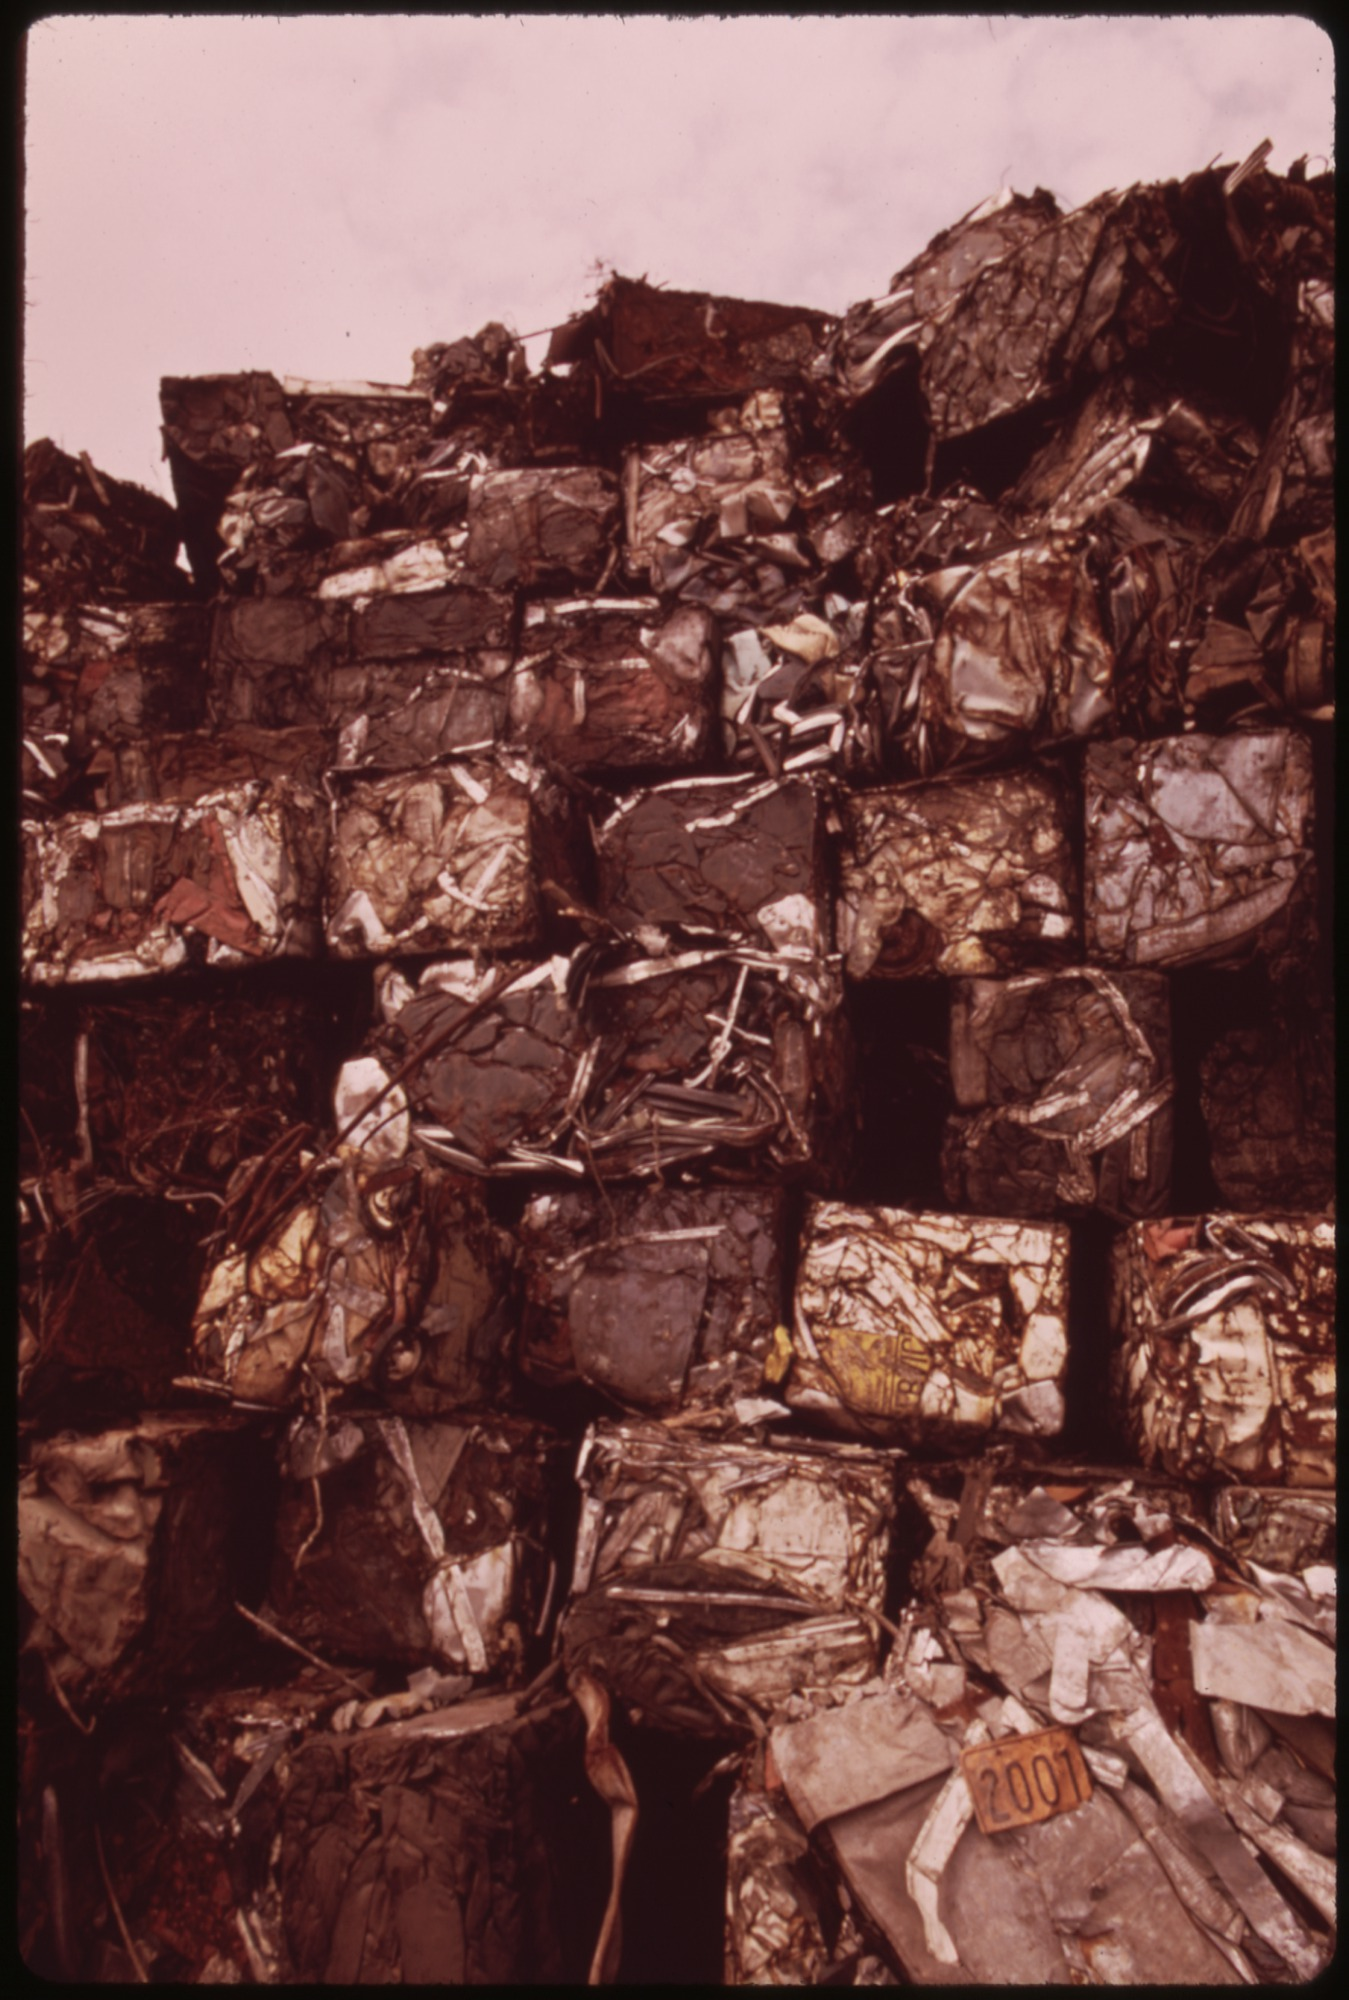
\includegraphics[width=\linewidth]{images/stack.jpg}
			
		\column{.7\linewidth}
			\begin{itemize}
				\item Kann mit \texttt{deque}, \texttt{list} und \texttt{vector} arbeiten
				\item Wichtig: \texttt{top()}, \texttt{push()} und \texttt{pop()}
				\item Laufzeit: $\mathcal{O}(1)$ für alle Einzel-Operationen
			\end{itemize}
			
			\vspace{1em}
			
			\begin{itemize}
				\item Einsatz: Bei Bedarf
			\end{itemize}
	\end{columns}
\end{frame}

\begin{frame}{\texttt{queue}}
	\begin{center}
		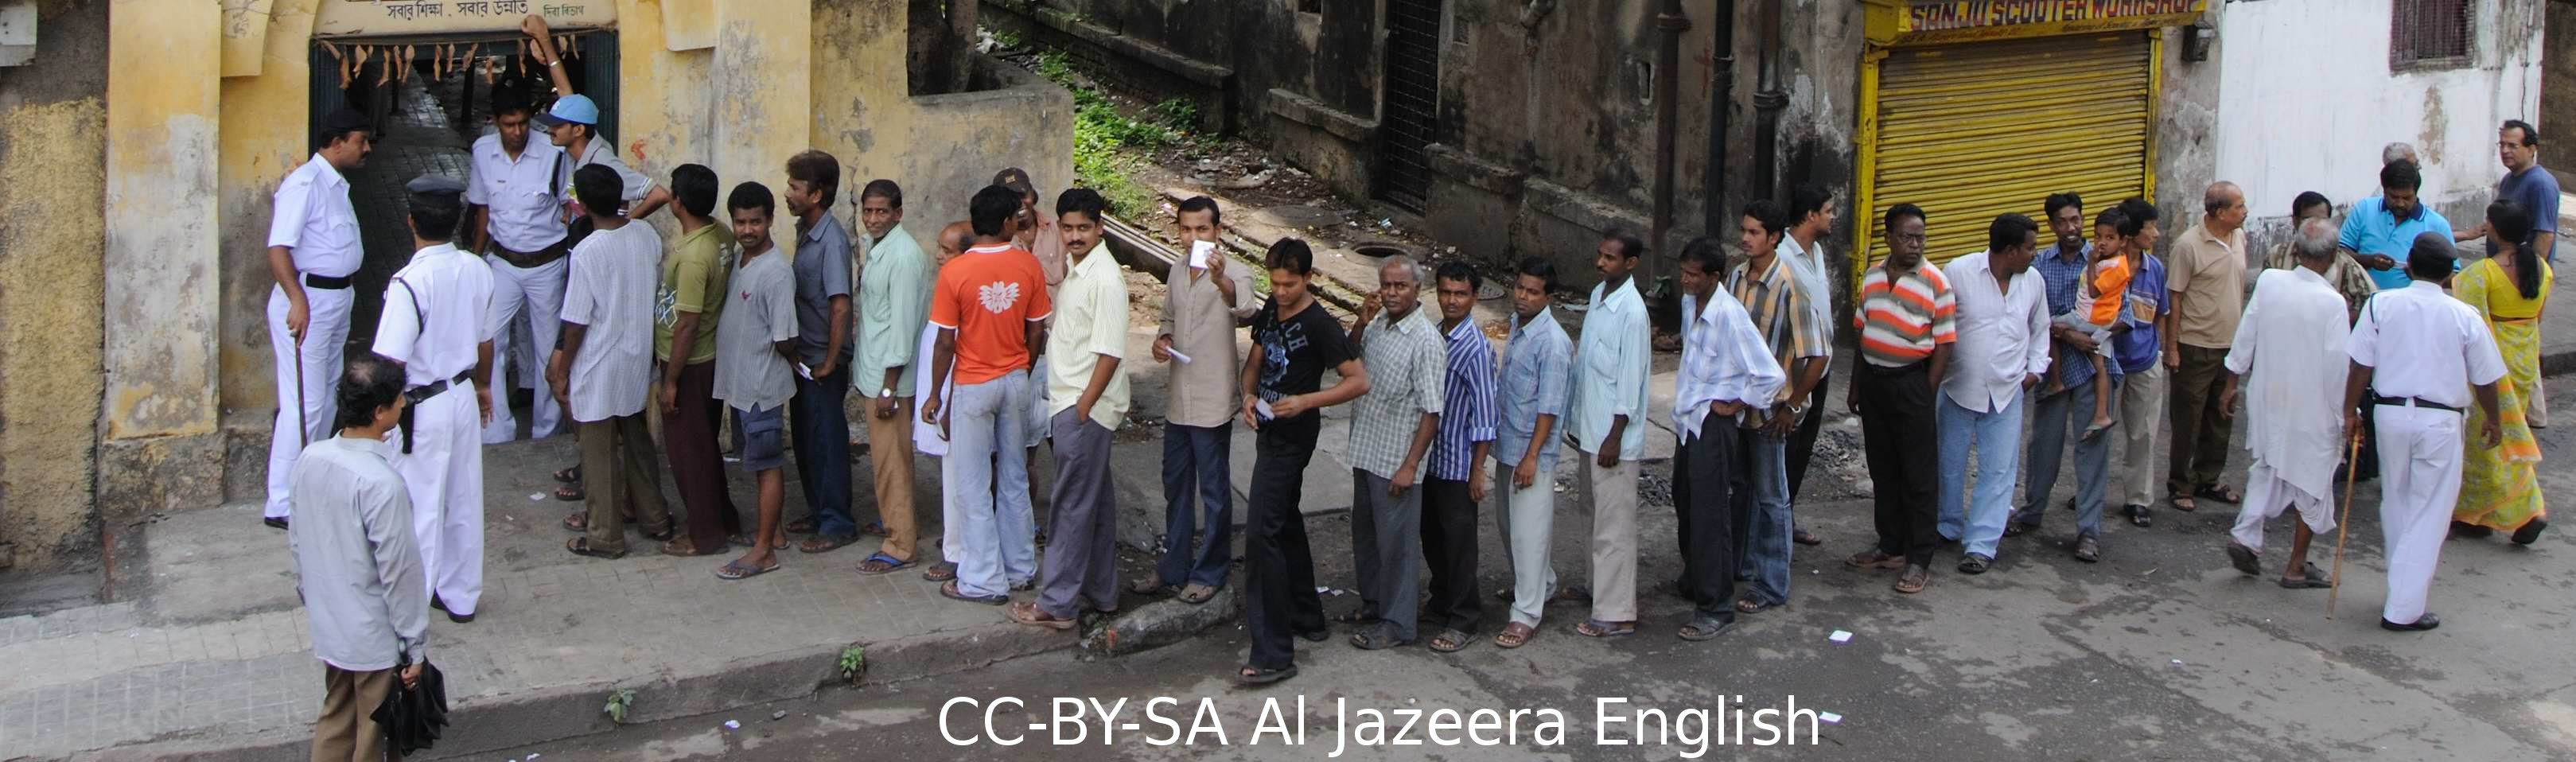
\includegraphics[width=0.7\linewidth]{images/queue.jpg}
	\end{center}
	
	\begin{itemize}
		\item Kann mit \texttt{deque} und \texttt{list} arbeiten, aber nicht mit \texttt{vector}
		\begin{itemize}
			\item \alert{Warum?}
			\pause
			\item Weil entfernen am Anfang eines \texttt{vector} \enquote{teuer} ($\mathcal{O}(n)$) ist
		\end{itemize}
		\item Wichtig: \texttt{front()}, \texttt{back()}, \texttt{push()} und \texttt{pop()}
		\item Laufzeit: $\mathcal{O}(1)$ für alle Einzel-Operationen
	\end{itemize}
	
	\begin{itemize}
		\item Einsatz: Bei Bedarf
	\end{itemize}
\end{frame}

\begin{frame}{\texttt{priority\_queue}}

\end{frame}

\subsection{associative containers}

\begin{frame}{Überblick}

\end{frame}

